\chapter{Datasets}
\label{ch:datasets}

\section{Fake Vs Real Expressions}

The first experiments were conducted using the SASE-FE database \cite{Ofodile2017AutomaticEmotion}. This dataset consists of 643 different videos. A total of 50 subjects participate. The participants have a range of age between 19 to 36. The dataset uses the six universal expressions: Happiness, Sadness, Anger, Disgust, Contempt and Surprise. Each participant in the dataset has two facial expressions of emotions, a genuine and a deceptive. 

% FIGURE: emotions
\begin{figure}[H]
     \begin{center}
%
        \subfigure[Fake Anger]{%
            \label{fig:real-fake_fake_anger}
            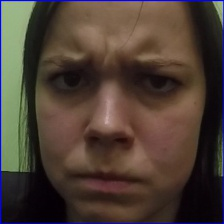
\includegraphics[width=0.32\textwidth]{anger_fake.jpg}
        }%
        \subfigure[Real Anger]{%
           \label{fig:real-fake_real_anger}
           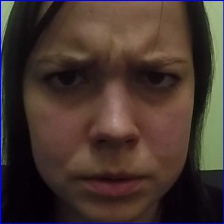
\includegraphics[width=0.32\textwidth]{anger_real.jpg}
        }
%
    \end{center}
    \caption{%
        Genuine and Deceptive emotions example in Fake vs Real Expressions dataset.
     }%
   \label{fig:fakedataset_fake-real_subfigures}
\end{figure}

The dataset has been split into training and test set. The training consists of the 80\% of the videos, while the validation test consists of 10\% of the videos and the test set consists also of 10\%. The training set consists of the videos of 40 participants, while the validation set consists of videos of 8 participants.

% FIGURE: emotions
\begin{figure}[H]
     \begin{center}
%
        \subfigure[Anger]{%
            \label{fig:fake_anger}
            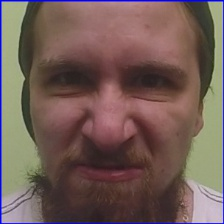
\includegraphics[width=0.25\textwidth]{fake_anger.jpg}
        }%
        \subfigure[Contentment]{%
           \label{fig:fake_contentment}
           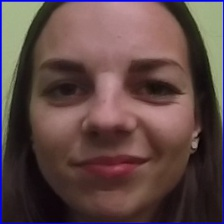
\includegraphics[width=0.25\textwidth]{fake_contentment.jpg}
        }%
        \subfigure[Disgust]{%
            \label{fig:fake_disgust}
            
\includegraphics[width=0.25\textwidth]{fake_disgust.jpg}
        }\\ %  ------- End of the first row ----------------------%
        \subfigure[Happiness]{%
            \label{fig:fake_happiness}
            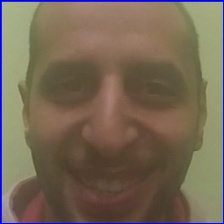
\includegraphics[width=0.25\textwidth]{fake_happiness.jpg}
        } %
        \subfigure[Sadness]{%
            \label{fig:fake_sadness}
            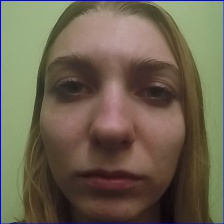
\includegraphics[width=0.25\textwidth]{fake_sadness.jpg}
        }%
        \subfigure[Surprise]{%
            \label{fig:fake_surprise}
            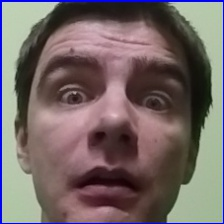
\includegraphics[width=0.25\textwidth]{fake_surprise.jpg}
        }
%
    \end{center}
    \caption{%
        Six universal emotions example in Fake vs Real Expressions dataset.
     }%
   \label{fig:fakedataset_subfigures}
\end{figure}

\section{Blocked Emotions}

Text of Datasets.